% !TEX root = main.tex

\section{物理层}
在\textbf{直连网}中传输原始比特流,不管包。
需要做的事情:
\[\text{信息源}\to\text{调制/编码}\to\text{信道传输}\to\text{解调/解码}\to\text{目的地}\]
其中调制解调为模拟信号,编码解码为数字信号。

信息能够被解释为数据(data),用符号(sign)记录,用信号(signal)(光、电)传递(transmit),用熵(entropy)测量。
\begin{itemize}
	\item 模拟信号-传输:连续取值(连续波长而不是连续信息),放大器(amplifier)
	\item 数字信号/跳变信号-传输:离散取值,中继器(repeater)
\end{itemize}

\subsection{编码方式}
\subsubsection{模拟信号}
载波信号(carrier)一般采用正弦波信号:角频率$\omega$、频率$f$、周期$T$、振幅$A$、相位$\varphi$
\begin{itemize}
	\item 频移键控(frequency-shift keying, FSK):通过不同频率表示不同信息0/1
	\item 幅移键控(amplitude-shift keying, ASK):通过不同振幅表示不同信息
	\item 相移键控(phase-shift keying, PSK):通过不同相位表示不同信息
	\item 正交调幅(quadrature amplitude modulation, QAM):用不同的\textbf{振幅和相位的组合}表示不同的多位信息,如$000\thicksim 111$
\end{itemize}

\subsubsection{数字信号}
\begin{enumerate}
\item 单极编码(unipolar):0V即0,$+E$V为1,但是会产生两种漂移
\begin{itemize}
	\item 时钟漂移:发送方和接收方采用\textbf{不同的时钟信号},或长时间没有校正信号;一定要有跳变
	\item 基线漂移:线很长会有,长时间传输\textbf{相同电平信号}导致积累很多\textbf{同种电荷},最后导致信号整体偏离基准线;一定要有变化/正负
\end{itemize}
\item 不归零编码/双极编码(non-return-to-zero/bipolar, NRZ) :$-E$为0,$+E$为1,解决基线漂移问题(平衡01);全是0或全是1,还是没法区分
\item 不归零反转编码(Inverted, NRZI):\textbf{差分}码波形,相邻码元的电位改变表示1,而电位不改变表示0;也可以反过来。 该表示方法与码元本身电位或极性无关,而仅与相邻码元的电位变化有关
\item 曼彻斯特(Manchester)编码:从相邻时刻的中间起降$-E\thicksim +E$,$0\to 10, 1\to 01$,\textbf{可克服时钟漂移和基线漂移};频率高,传输有问题,对传输介质要求高
\item 差分曼彻斯特编码:在每一位开始时间如果跳变(当前编码与原数据不同)则为0,否则为1,且中间也要跳变
\begin{figure}[H]
	\centering
	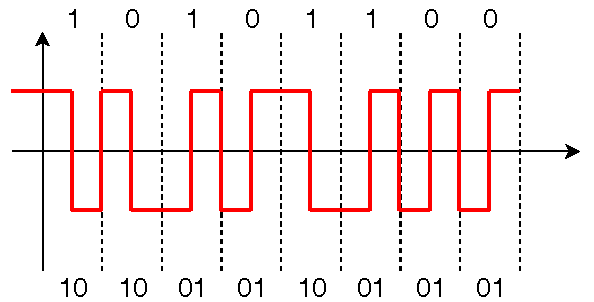
\includegraphics[width=0.5\linewidth]{fig/network-manchester.pdf}
\end{figure}
\item 4B/5B编码:用5比特代表4比特,多一位冗余;每个编码没有多于1个前导零和多于2个末端零,即\textbf{最多3个0};防止跳变过多,又可消除基线漂移和时钟漂移
\begin{center}
\begin{tabular}{|c|c||c|c|}\hline
4B & 5B & 4B & 5B\\\hline\hline
0000 & 11110 & 1000 & 10010\\\hline
0001 & 01001 & 1001 & 10011\\\hline
0010 & 10100 & 1010 & 10110\\\hline
0011 & 10101 & 1011 & 10111\\\hline
0100 & 01010 & 1100 & 11010\\\hline
0101 & 01011 & 1101 & 11011\\\hline
0110 & 01110 & 1110 & 11100\\\hline
0111 & 01111 & 1111 & 11101\\\hline
\end{tabular}
\end{center}
\end{enumerate}

\subsection{物理介质}
\subsubsection{分类}
\begin{enumerate}
\item 有线介质
\begin{itemize}
	\item 双绞线:
	\begin{itemize}
		\item 非屏蔽双绞线(unshielded twisted pair, UTP):四对线(绿绿白、橙橙白、蓝蓝白、棕棕白),cat5/cat5e百兆以太网,cat6千兆以太网\footnote{1KB(Kilobyte,千字节),1MB(Megabyte,兆字节,简称``兆''),1GB(Gigabyte,吉字节,又称``千兆'')}
		\item 屏蔽双绞线(STP)
	\end{itemize}
	\item 同轴电缆(coaxial cable)
	\item 光导纤维(optical fiber):利用光的全反射性质
	\begin{itemize}
		\item 单模光纤(single mode):最大传输速率
		\item 多模光纤:阶跃(step-index)光纤、渐变(graded-index)光纤
	\end{itemize}
\end{itemize}
\item 无线介质:地面微波、WiFi、3G网络、卫星
\end{enumerate}

\subsubsection{多路复用}
\begin{itemize}
	\item 时分多路复用(time division multiplexing, TDM):时间域被分成周期循环的一些小段,每段时间长度是\textbf{相同}的,每个时段用来传输一个子信道
	\item 频分多路复用(frequency, FDM):\textbf{无线电台}常用
	\item 波分多路复用(wavelength, WDM):利用多个激光器在单条光纤上同时发送多束不同波长激光的技术
	\item 码分多路复用(code, CDM):利用各路信号码型结构正交性而实现多路复用
	\item 统计多路复用(static, SDM):\textbf{动态分配}方法共享通信链路,比如FIFO;对于多个\textbf{可变速率}的数据流,SDM可以提高链路利用率
\end{itemize}

% 如果有8个速率相同的数据流,且它们速率之和小于且接近一条链路的带宽,与用8个通道(channel)的TDM或FDM传送它们相比,采用统计多路复用技术的带宽利用率(传送有效数据的比率)怎么样?
% 更差,都可以用完整个带宽,只是统计复用技术需要地址,因此会差一点